\section{Object Detection Datasets}
\label{sec:ObjectDetectionDatasets}

% ##################################################
\subsection{MS COCO}
\label{ssec:DatasetMSCOCO}

The \datasetname{MS \gls{coco}} dataset~\cite{Lin2014} (web:~\cite{mscocodataset}) was created for the purpose of object segmentation. However, if a model solves a much more complicated problem of object segmentation, pure object detection is then just one of many steps. To this end, this dataset is often adopted for training object detectors. It is a widely used dataset for image classification, object detection, and semantic segmentation. It is considered a benchmark dataset in different academic and industrial research areas. The images in the dataset are everyday objects captured from everyday scenes. This adds some “context” to the objects captured in the scenes.

\begin{figure}[t]
    \centerline{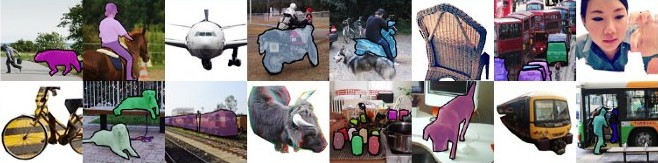
\includegraphics[width=\linewidth]{figures/datasets/ms_coco_sample.jpeg}}
    \caption[\datasetname{MS \gls{coco}} dataset]{The \datasetname{MS \gls{coco}} dataset provides $80$ classes ($81$ if background is taken into account) of common objects in everyday life, which brings an additional contextual information. \externalsrc{\cite{mscocodataset}}}
    \label{fig:DatasetMSCOCO}
\end{figure}

% ##################################################
\subsection{KITTI Object Detection}
\label{ssec:DatasetKITTIObjectDetection}

The \datasetname{KITTI Object Detection} dataset~\cite{Geiger2012CVPR} (web:~\cite{kittiobjectdetectiondataset}) can be adopted for training models for object detection and object orientation estimation. This benchmark holds $7\ 481$ training images and $7\ 518$ test images, comprising a total of $80\ 256$ labeled objects. This work is of significant value for our research because of a firm ground for building an object detector aimed at traffic applications. Classes of objects are "car", "van", "truck", "pedestrian", "person sitting", "cyclist", "tram", "miscellaneous" or "don't care". Besides the rich content of traffic-related objects, additional information such as object and camera real-world positions are available, too. As we have mentioned the goal of dealing with object occlusion, this dataset provides an occlusion tag that represents the level of occlusion, from full visibility to large occlusion.

\begin{figure}[t]
    \centerline{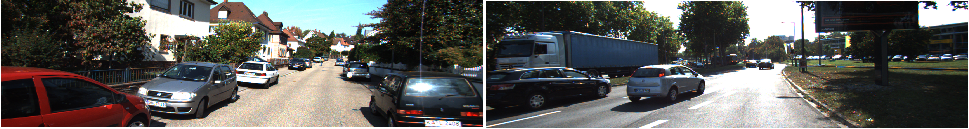
\includegraphics[width=0.9\linewidth]{figures/datasets/kitti_detection_sample.pdf}}
    \caption[\datasetname{KITTI Object Detection} dataset]{The \datasetname{KITTI Object Detection} dataset provides traffic-related, unconstrained scenarios with full details about the scene: object \glspl{bbox}, camera and object positions as well as indicators of occlusion level. \externalsrc{\cite{Geiger2012CVPR}}}
    \label{fig:DatasetKITTIDetection}
\end{figure}
